\newpage

\subsection{Configuration for code generation in Eclipse}
\visHeader

As there is already generated code (provided via a plugin in Eclipse) for the existing \texttt{GenModel} metamodel, we do \emph{not} want to export our
incomplete subset of \texttt{GenModel} in EA.

\begin{enumerate}
\item[$\blacktriangleright$] To prevent this, right-click the \texttt{GenModel} package in EA and select ``Properties/Moflon'' and change the tagged value
\texttt{Moflon::Export} to \texttt{false} (Fig.~\ref{fig_customNS}).
\end{enumerate}

\begin{figure}[htb]
\begin{center}  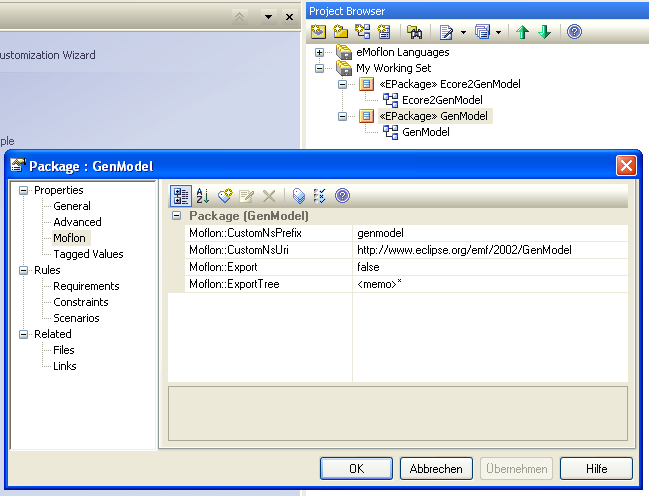
\includegraphics[width=\textwidth]{8_nsUriPre_edited}
  \caption{Update the \texttt{GenMode} export option and create custom tags}  
  \label{fig_customNS}
\end{center}
\end{figure}

Furthermore, we have to set the ``real'' name and URI of the project to be used in Eclipse so that references are exported properly. 

\begin{enumerate}

\item[$\blacktriangleright$] In the ``Properties/Moflon" dialogue for \texttt{GenModel}, create the new tagged values \texttt{Moflon::CustomNsPrefix} and
\texttt{Moflon::CustomNsUri} and set them according to Fig.~\ref{fig_customNS}. These values can be determined by inspecting the corresponding values in the
existing .ecore file (i.e.,~the existing metamodel).

\item[$\blacktriangleright$] Export all projects as usual to your Eclipse workspace and update the metamodel project by pressing \texttt{F5}.

\item[$\blacktriangleright$] Convert the generated Eclipse project \texttt{Ecore2GenModel} to a \emph{plugin project} by right-clicking the project and
selecting ``Configure/Convert to Plug-in Projects...''. This makes it easier to set the required dependencies for code generation.

\item[$\blacktriangleright$] Now right-click \texttt{Ecore2GenModel} and choose ``Plug-in Tools/Open Manifest''. In the window that opens up, choose the
\texttt{Dependencies} tab, click \texttt{Add}, and type in \texttt{org.eclipse.emf.codegen.ecore} (which includes both the \texttt{Ecore} and \texttt{GenModel}
libraries as required).

\end{enumerate}

Although we have already specified the name and URI of the existing project (in our case \texttt{GenModel}) in EA, we now have to tell eMoflon where to find the
implementation (generated code) for the existing project.

\begin{enumerate}
\item[$\blacktriangleright$] Open the \texttt{moflon.properties} file located in your project folder and insert the following lines:\\
\end{enumerate}

\vspace{-1cm}
{\small \ttfamily \hspace{-2.5cm} ADDITIONAL\_DEPENDENCIES=platform:/plugin/org.eclipse.emf.codegen.ecore/model/GenModel.ecore} \\
\vspace{0.75cm}%
{\small \ttfamily \hspace{-2.5cm} ADDITIONAL\_USED\_GEN\_PACKAGES=platform:/plugin/org.eclipse.emf.codegen.ecore/model/GenModel.genmodel}

Finally, to compenstate for some cases where our naming conventions were violated, add the following mappings as corrections:

\begin{enumerate}
\item[$\blacktriangleright$] An \emph{import mapping} for correct generation of the required import:

{\small \ttfamily IMPORT\_MAPPINGS=genmodel-> org.eclipse.emf.codegen.ecore.genmodel}


\item [$\blacktriangleright$] A \emph{factory mapping} to ensure that \texttt{GenModelFactory} is used as the factory for creating elements in the
transformation instead of \texttt{Genmodel\-Factory}, which would be the default convention:

{\small \ttfamily FACTORY\_MAPPING=genmodel-> GenModelFactory}

\end{enumerate}


\newpage

Your \texttt{moflon.properties} file should now closely resemble Fig.~\ref{fig_mofProp}. Generate code one more time for the project and ensure (with a JUnit
test) that the transformation behaves as expected.

\vspace{0.5cm}

\begin{figure}[htbp]
\hspace*{-2cm}
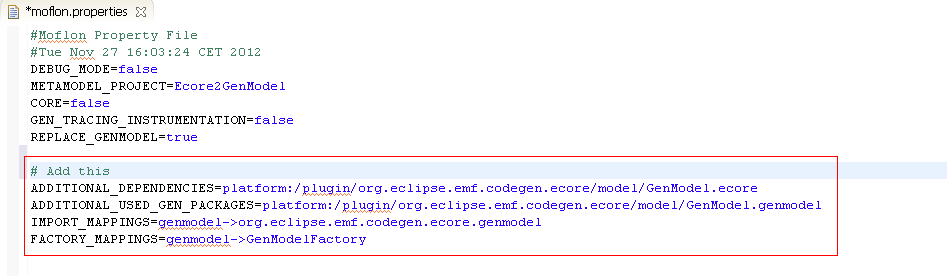
\includegraphics[width=1.5\textwidth]{9_mofProperties}
  \caption{Additional properties for code generation}  
  \label{fig_mofProp}
\end{figure} 
